\documentclass{article}
\usepackage[english]{babel}
\usepackage[letterpaper,top=2cm,bottom=2cm,left=3cm,right=3cm,marginparwidth=1.75cm]{geometry}
\usepackage{amsmath}
\usepackage{graphicx}
\usepackage[colorlinks=true, allcolors=blue]{hyperref}
\usepackage[numbers]{natbib}
\usepackage{listings}
\usepackage{subcaption}

\setlength{\textfloatsep}{8pt plus 2pt minus 2pt}
\setlength{\floatsep}{8pt plus 2pt minus 2pt}
\setlength{\intextsep}{8pt plus 2pt minus 2pt}

\title{NOvA Production 6 Validation Task Force Contribution Summary}
\author{Thiago Bezerra (Sussex)}

\begin{document}
\maketitle

\section{Task Description}

My contribution to the Production~6 Validation Task Force was to validate the
mass-produced \textbf{cosmic-ray sample}, comparing the new Prod6 against the
previous Prod5.1. The validation overlays the distributions of a large set of
reconstructed variables, spanning the full reconstruction chain from low-level
(slice) quantities up to the final analysis observables, both summed over all
quantiles and split by quantile, applying the standard 3-flavor FD veto cuts
(\texttt{kStandardSpillCuts \&\& kNumuBasicQuality \&\& k3flavor2024FDVeto}).
To make the comparison robust, dedicated SAM definitions were prepared so that
both productions use the \emph{same} runs/subruns and livetime, removing apparent
differences from comparing different exposures. Two run ranges were studied (600
files each): an early range ($973.011$\,s, runs $[13458, 14501]$) and a later range
($209.847$\,s, runs $[47191, 47238]$); they share the same base definition per
production, differing only in the \texttt{prestage} suffix (in braces below, early
then later):
{\footnotesize
\begin{itemize}
  \setlength{\itemsep}{1pt}
  \item Prod6:
  \texttt{prod\_\allowbreak caf\_\allowbreak R25-06-04-prod6.h\_\allowbreak fd\_\allowbreak cosmic\_\allowbreak full\_\allowbreak v1\_\allowbreak Prod6\_\allowbreak official\_\allowbreak prestage\_\allowbreak \{1780583415,\,1781173252\}}
  \item Prod5.1:
  \texttt{prod\_\allowbreak caf\_\allowbreak R20-11-25-prod5.1reco.q.t\_\allowbreak fd\_\allowbreak cosmic\_\allowbreak fhc\_\allowbreak allperiods\_\allowbreak v1\_\allowbreak goodruns\_\allowbreak nostale\_\allowbreak bad\_\allowbreak cosmics\_\allowbreak removed\_\allowbreak prestage\_\allowbreak \{1780502924,\,1781172704\}}
\end{itemize}
}
The analysis scripts live in the \texttt{novasoft}
branch \texttt{feature/tbezerra\_cosmic\_pred6\_comp} under
\texttt{3FlavorAna/\allowbreak Ana2024/\allowbreak Cosmics/\allowbreak prod6Validation}.
The work was reported in two talks and a follow-up slides: the first check~\cite{docdb-69724},
a follow-up update~\cite{docdb-70051}, and the latest update~\cite{docdb-70174}.

\section{Findings}

The large majority of variables agree well: slice-level quantities and
Kalman-track variables have the same distributions in both prods, and, most
importantly, the final analysis observables (reconstructed neutrino, muon and
hadronic energies) are consistent. A handful of discrepancies were identified and
followed up:

\begin{itemize}
  \item \textbf{Empty vertex / BPF variables in Prod6 (resolved).} During the
  first look, several vertex and BPF variables came out
  empty in Prod6 because the vertexing moved from ElasticArms to MLVertex; once
  pulled from MLVertex they are populated again. The remaining vertex and BPF
  shape differences (e.g.\ Fig.~\ref{fig:tbezerra-vtx-remid}, left) are small and
  expected from the new vertexing.

  \item \textbf{CosRej time dependence.} The cosmic-rejection (CosRej) score does
  not match between the two productions, and the level of disagreement depends on
  the run period (Fig.~\ref{fig:tbezerra-cosrej}). This is also present for the
  $\nu_e$ CosRej. P1/P2 use hard-coded weight files for the numu CosRej BDT, so an
  open question is whether the BDT was re-trained for Prod6 from P3 onwards.

  \item \textbf{remID / Scattering LLH.} The remID PID shows a difference between
  the two productions (Fig.~\ref{fig:tbezerra-vtx-remid}, middle). Checking its
  inputs, the only one that disagrees is the muon scattering log-likelihood
  (Scattering LLH, Fig.~\ref{fig:tbezerra-vtx-remid}, right), pointing to a change
  in the muon scattering PDF for Prod6.
\end{itemize}

\begin{figure}[t]
    \centering
    \begin{subfigure}{0.32\textwidth}
        \centering
        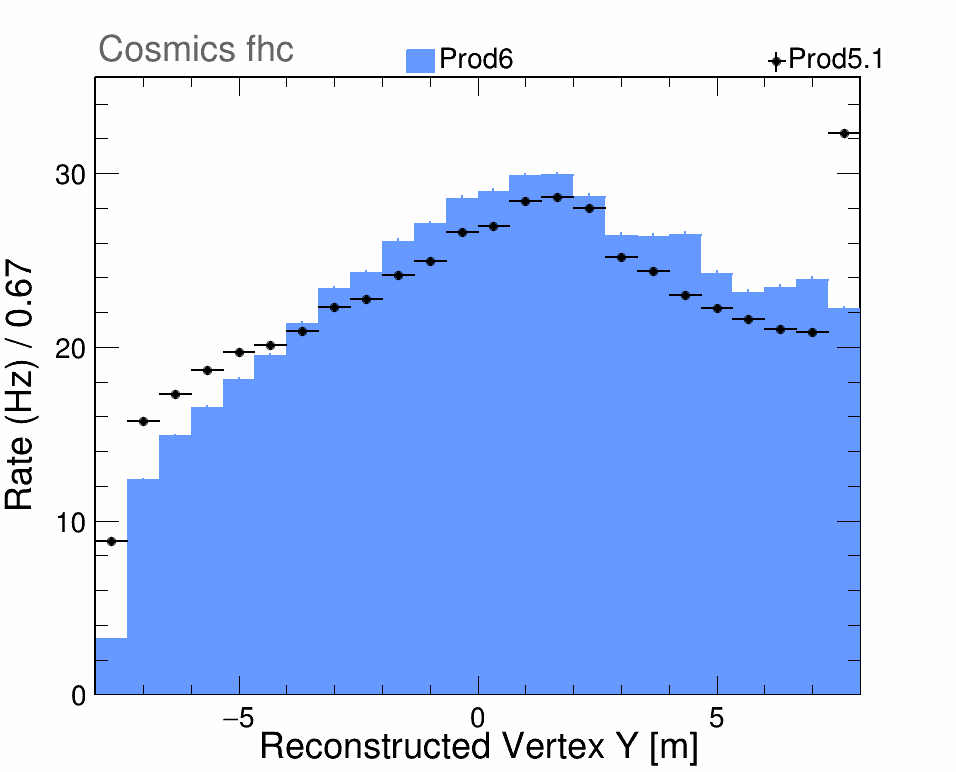
\includegraphics[width=\textwidth]{images-tbezerra/vtxY.png}
        \caption{Vertex $Y$ (MLVertex)}
    \end{subfigure}
    \hfill
    \begin{subfigure}{0.32\textwidth}
        \centering
        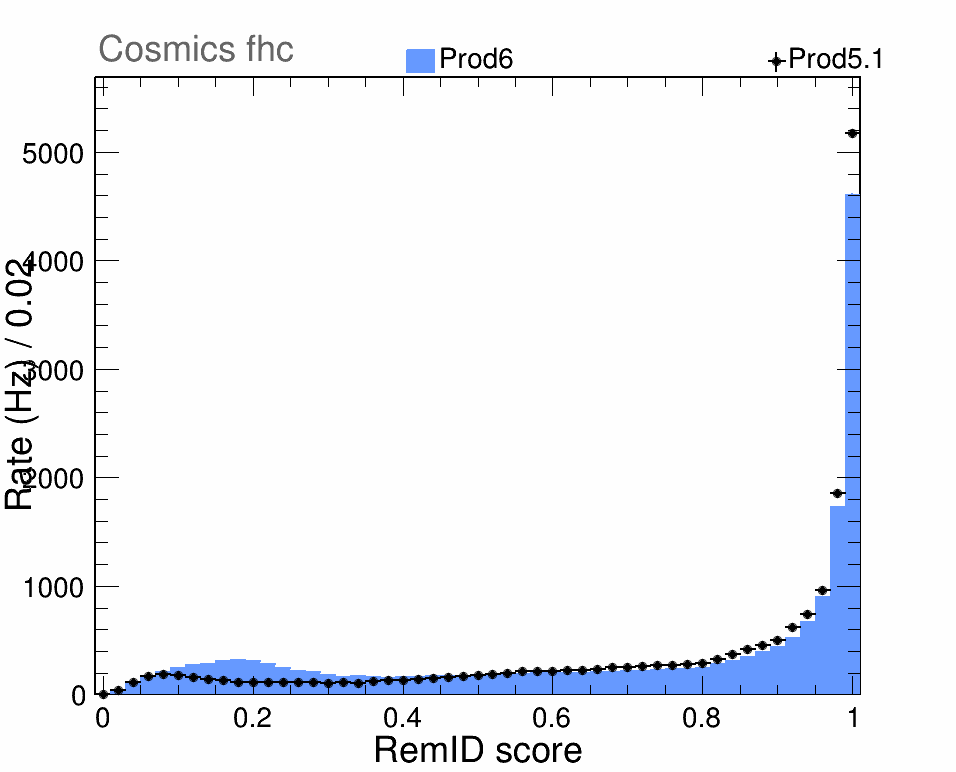
\includegraphics[width=\textwidth]{images-tbezerra/remID.png}
        \caption{remID}
    \end{subfigure}
    \hfill
    \begin{subfigure}{0.32\textwidth}
        \centering
        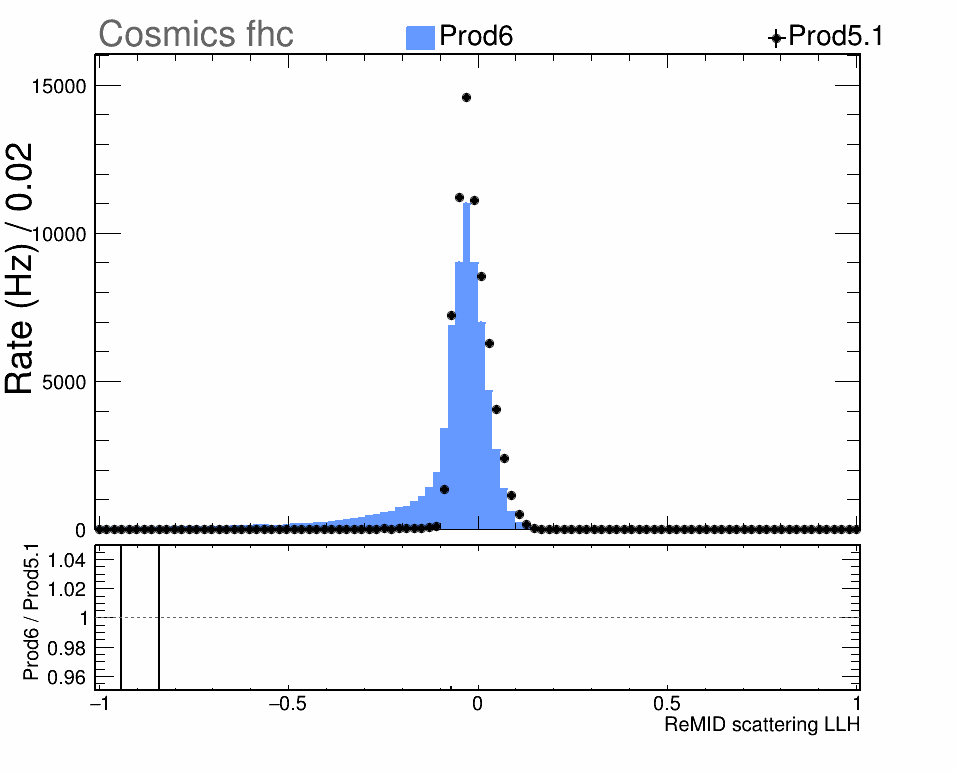
\includegraphics[width=\textwidth]{images-tbezerra/remIdScatLLH.png}
        \caption{remID Scattering LLH}
    \end{subfigure}
    \caption{Left: vertex $Y$ recovered from MLVertex, showing the small expected
    difference after the ElasticArms\,$\rightarrow$\,MLVertex
    change~\cite{docdb-70051}. Middle: the remID PID differs between
    productions; right: its only discrepant input is the muon scattering
    log-likelihood~\cite{docdb-70174}.}
    \label{fig:tbezerra-vtx-remid}
\end{figure}

\begin{figure}[t]
    \centering
    \begin{subfigure}{0.42\textwidth}
        \centering
        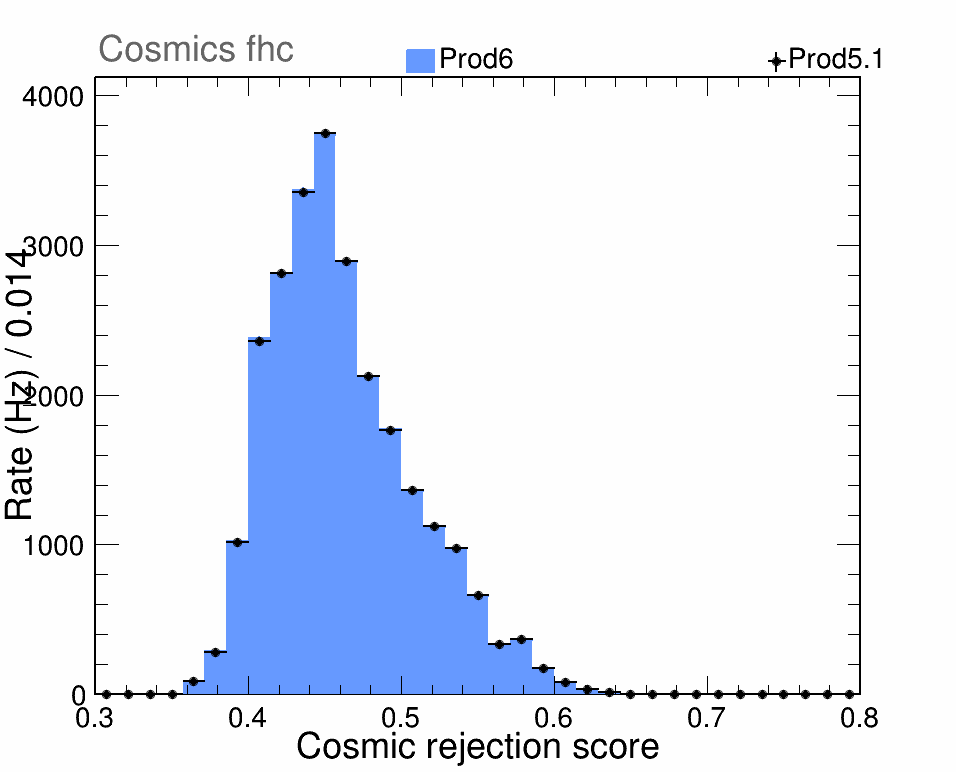
\includegraphics[width=\textwidth]{images-tbezerra/cosRej_runs13458-14501.png}
        \caption{Runs $[13458, 14501]$}
    \end{subfigure}
    \hfill
    \begin{subfigure}{0.42\textwidth}
        \centering
        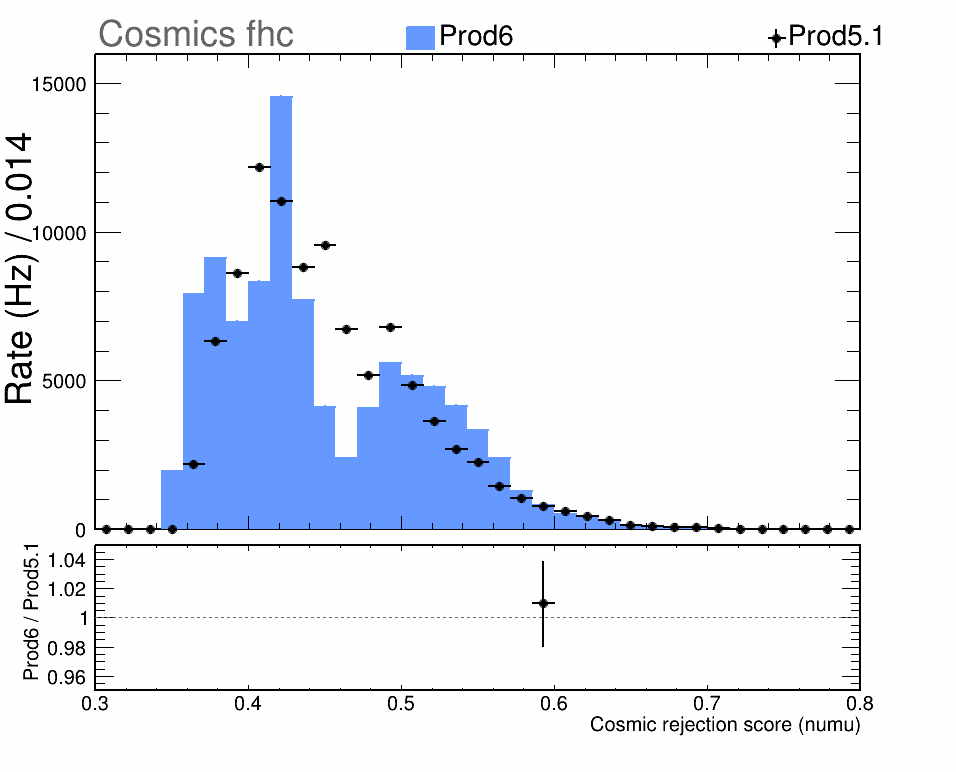
\includegraphics[width=\textwidth]{images-tbezerra/cosRej_runs47191-47238.png}
        \caption{Runs $[47191, 47238]$}
    \end{subfigure}
    \caption{CosRej ($\nu_\mu$) score for Prod6 vs Prod5.1 on same-run definitions,
    for two different run ranges. The level of disagreement changes with the run
    period, indicating a temporal dependence of the cosmic-rejection
    score~\cite{docdb-70174}.}
    \label{fig:tbezerra-cosrej}
\end{figure}

\section{A Complete List of Relevant Docdbs with Citations Including URL}

\noindent\cite{docdb-69724}~--~First check of cosmics from Prod6, the preliminary
results first shown to the collaboration (May~2026). Key plots: agreement of the
final analysis observables (recoE), the first CosRej and remID discrepancies, and
the empty BPF/vertex variables later traced to the ElasticArms\,$\rightarrow$\,MLVertex change.

\noindent\cite{docdb-70051}~--~Follow-up update introducing the same-run
definitions (CM Parallel~7). Key plots: the recovered MLVertex and BPF variables
and their small, expected residual differences.

\noindent\cite{docdb-70174}~--~Latest update of the study. Key plots: the CosRej
time dependence across run periods, inclusion of $\nu_e$ CosRej, and the remID Scattering LLH
mismatch; the comparison for the complete list of variables is in this document's backup.

\bibliographystyle{unsrtnat}
\bibliography{summary-tbezerra}

\end{document}
